
\chapter{CONTROLLERS}
\label{chap:Controllers}

The control requirements for NASA MMS TableSat IA can be simplified into three main goals.

The first is to maintain a steady spin rate of 3 rpm ($\pi/10$ rad/sec).  Given the relative success of the body rate estimation in Chapter \ref{chap:Estimators}, this goal should be attainable without the need of advanced control efforts.

The second is to correct for any nutation wobble about the $x$ and $y$ body axes.  This requirement essentially can be seen as driving body rates $\omega_y$ and $\omega_z$ to zero and ensuring the estimated quaternion's Euler axis is kept in line with the global reference frame's $z$-axis.

The third is to prevent and/or remove oscillations in the Axial Double Probe (ADP) and Spin-plane Double Probe (SDP) booms.  Out of the three, this performance goal has the largest set of dependencies for success.  This level of control is reliant on effective actuators along with reliable state estimates based on an accurate system model which include flexible boom dynamics.

The first two goals are addressed in this chapter as their scope is limited to controller design.  Section \ref{sec:ActuatorConfiguration} covers the configuration of the actuators on TableSat and how their configuration is incorporated into the controller code.  The remaining sections of this chapter focus on rate and nutation control methods.  In this part of the research it is assumed that the estimators provide perfect state estimates.  These conditions temporarily limit the scope of the testing to ensure that the control techniques are being implemented properly in the software especially since with the development of some non-standard techniques.  The third goal, controlling boom oscillations, is addressed in Chapter \ref{chap:ObserverBasedControls} when multiple modules are linked together to obtain a wider view of the interactions between observer-based controllers being acted upon by noisy state measurements.

\section{Actuator Configuration}
\label{sec:ActuatorConfiguration}

As shown in Figure \ref{fig:TSatThrusters}, the actuators on NASA MMS TableSat IA consist of four single directional computer fans.  Two are oriented for rate control and two for nutation control.  The body rate control fans are mounted on opposite sides of the bus with their thrusts applying opposing moments.  The two nutation fans are mounted flush with the bus at a 90 degree offset and have their thrust directed downward.  The fans are assumed to be mounted such that the moments are applied about orthogonal axes.  This simplifies the actuator module's voltage input calculations for each fan which can be improved if testing shows that the effects from the off center are significant enough to compensate for.  Four analog ports to the Athena PC are available for actuator usage after mounting the sensors.  Two are dedicated to the rotational fans to provide full rotational control, and the remaining two provide limited nutation control.
\begin{figure}[H]
  \centerline{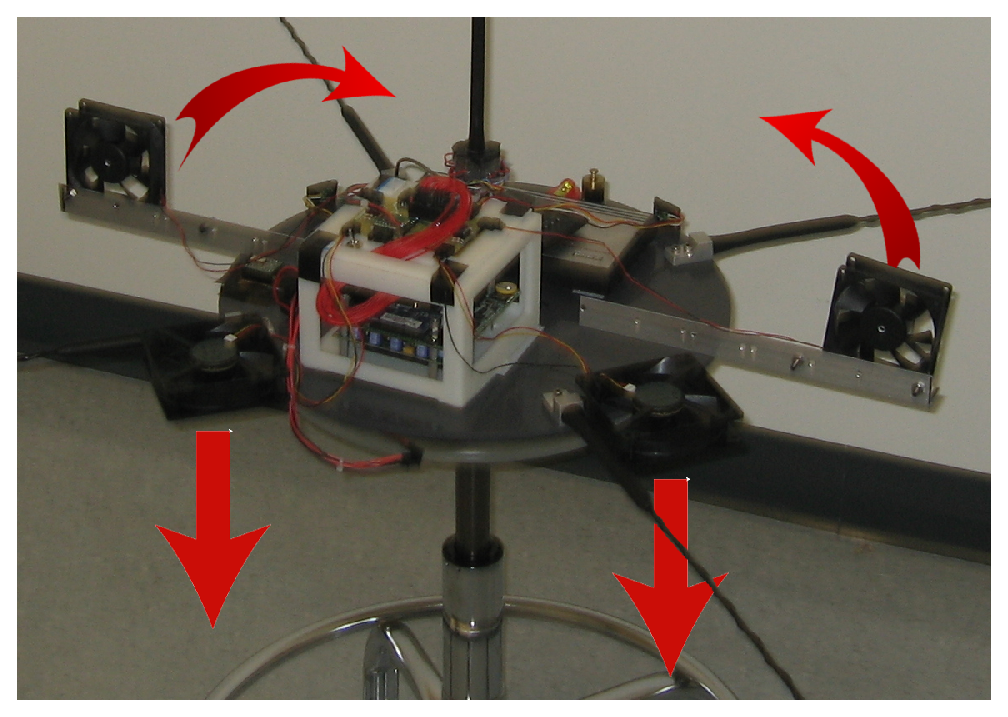
\psfig{file=figures/tsat_thrusters.eps,height=3in}}
  \caption{NASA MMS TableSat IA thrusters}
  \label{fig:TSatThrusters}
\end{figure}
Sending the desired moment control commands from the controller directly to the estimator without taking the fan geometry into consideration creates a disconnect between the estimated and actual system states.  The software's actuator module is designed to accept a list of fans with their center, direction of thrust related to the body reference frame, and maximum force to determine the moments couples that are actually possible.
\begin{figure}[H]
  \centerline{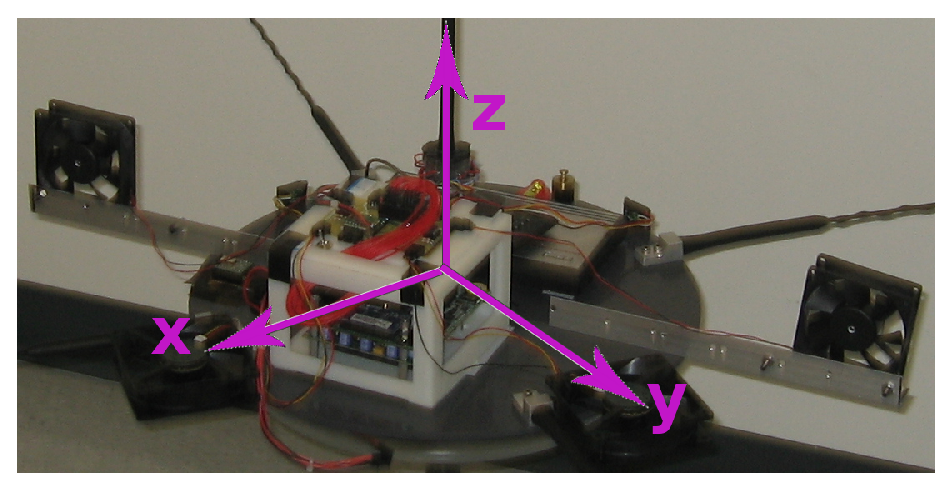
\psfig{file=figures/tsat_body_axes.eps,height=3in}}
  \caption{NASA MMS TableSat IA Body Axes}
  \label{fig:TableSatBodyAxes}
\end{figure}
Table \ref{tbl:ActuatorConfiguration} shows the fan configuration for the NASA MMS TableSat IA as arranged in Figure \ref{fig:TSatThrusters}.  Figure \ref{fig:TableSatBodyAxes} shows the body-fixed coordinate system.
\begin{table}[H]
  \centering
  \begin{tabular}{c|c|c|c|c}
    Fan & Center $\bs{f_c}$ (m) & Direction $\bs{n}$ & $F$ (N) & Max Moment $\frac{F \bs{n} \times \bs{f_c}}{|\bs{n}|}$ (Nm) \\ \hline
    1 & $(0.2474, -0.2474, 0)$ & $(-1, -1, 0)$ & 0.08 & $(0, 0, 0.039598)$ \\
    2 & $(-0.2474, 0.2474, 0)$ & $(-1, -1, 0)$ & 0.08 & $(0, 0, -0.039598)$ \\
    3 & $(0.25, 0, 0)$ & $(0, 0, -1)$ & 0.08 & $(0.02, 0, 0)$ \\
    4 & $(0, 0.25, 0)$ & $(0, 0, -1)$ & 0.08 & $(0, -0.02, 0)$ \\
  \end{tabular}
  \caption{Actuator configuration}
  \label{tbl:ActuatorConfiguration}
\end{table}
The algorithm shown in Snippet \ref{code:actuator_usage} demonstrates the actuator module's functionality implemented in the TSatPy software.  Lines 4-13 define the geometry of the actuators displayed in Figure \ref{fig:TSatThrusters} with the addition of a hypothetical fifth actuator along with their center, direction of thrust, and maximum thrust force.


\begin{listing}
\begin{singlespace}
  \begin{minted}[mathescape,linenos,numbersep=10pt,frame=lines,framesep=2mm]{python}
import numpy as np
from TSatPy.Actuator import Actuator

configs = [{'type': 'fan', 'args': {'name': 'CW',
  'center': (0.2474, -0.2474, 0), 'direction': (-1, -1, 0), 'F': 0.08}
},{'type': 'fan', 'args': {'name': 'CCW1',
  'center': (-0.2474, 0.2474, 0), 'direction': (-1, -1, 0), 'F': 0.08}
},{'type': 'fan', 'args': {'name': 'CCW2',
  'center': (-0.2474, -0.2474, 0), 'direction': (1, -1, 0), 'F': 0.08}
},{'type': 'fan', 'args': {'name': 'NY', 'center': (0.25, 0, 0),
  'direction': (0, 0, 1), 'F': 0.08}
},{'type': 'fan', 'args': {'name': 'NX', 'center': (0, 0.25, 0),
  'direction': (0, 0, 1), 'F': 0.08}}]

def set_level(act, power_level):
    print 'Setting power level=%g for: %s' % (power_level, act)

def setup_actuators(configs):
    act = Actuator()
    for config in configs:
        act.add(config['type'], set_level, config['args'])
    return act

act = setup_actuators(configs)
print(act)
M = np.mat([0.03, 0.11, 0.04]).T
print("Request moment: %s" % (M.T))
print("Applied moment: %s" % (act.request_moment(M).T))

# Prints Out
# Actuator
#  <Fan CW moment=(0, -0, -0.0279901)>
#  <Fan CCW1 moment=(0, 0, 0.0279901)>
#  <Fan CCW2 moment=(0, 0, 0.0279901)>
#  <Fan NY moment=(0, -0.02, 0)>
#  <Fan NX moment=(0.02, 0, 0)>
# Request moment: [[ 0.03  0.11  0.04]]
# Setting power level=1 for: <Fan NX moment=(0.02, 0, 0)>
# Setting power level=0.714538 for: <Fan CCW1 moment=(0, 0, 0.0279901)>
# Setting power level=0.714538 for: <Fan CCW2 moment=(0, 0, 0.0279901)>
# Applied moment: [[ 0.02  0.    0.04]]
  \end{minted}
\caption{Moment to actuator voltage conversion}
\label{code:actuator_usage}
\nocite{minted}
\end{singlespace}
\end{listing}

At line 24, the actuator instance is created and each fan's potential contribution to the overall control moment is calculated with
\begin{equation}
  \bs{M} = \frac{F \bs{n} \times \bs{f_c}}{|\bs{n}|}
\end{equation}
where the moment couple $\bs{M}$ is calculated from the max actuator force $F$, the direction of the thrust $\bs{n}$, and $\bs{f_c}$ is fan's center relative to the center of rotation.
The script output shown in Snippet \ref{code:actuator_usage} describes how a requested moment of $M_x = 0.03Nm, M_y = 0.11Nm, \text{ and } M_z = 0.04Nm$ is applied to the five-fan configuration.  The ``Nx'' fan can only produce a $0.02Nm$ moment, so it is set to full power to supply part of the requested $M_x = 0.03Nm$.  The ``Ny'' fan does not contribute since it's thrust is in the opposite direction from the needed $M_y = 0.11Nm$.  The ``CCW1'' and ``CCW2'' fans can not individually meet the requested $M_z = 0.04Nm$, but they are able to collaboratively reach the requested moment by contributing 71\% each.  In the end, the actual moment that is applied to the TableSat is $M_x = 0.02Nm, M_y = 0Nm, M_z = 0.04Nm$.  This actual moment is converted to equivalent voltage commands to be transmitted to the TableSat, and supplied to the estimator to propagate its dynamics.

\section{Rate Control}
\label{sec:RateControl}

The first of the three controls goals introduced at the start of this chapter is to control the TableSat to maintain a desired body rate of $\bs{\omega}_d$ such that
\begin{equation}
  \bs{\omega}_d = 0 \bs{i} + 0 \bs{j} + 0.314 \bs{k}
\end{equation}
This desired rate is used for the tests in Sections \ref{subsec:PRateControl} through \ref{subsec:SlidingModeController}.  As explained previously, all body rate controllers are tested under the assumption of perfect observer state feedback to ensure appropriate functionality before combining with other modules for observer-based control.
\subsection{P Rate Controller}
\label{subsec:PRateControl}
The initial controller tested is the proportional body rate controller of the form
\begin{equation}
  \bs{M}_{\omega} = \bs{K}_{\omega p} \left( \bs{\hat{\omega}} - \bs{\omega}_d \right)
  \label{eqn:PRateControl}
\end{equation}
Through a series of simulations with randomized initial conditions for body rates a gradient descent based on minimizing control effort is used to tune the proportional gains to
\begin{equation}
  \bs{K}_{\omega p} = \begin{bmatrix} 0.404 & 0 & 0 \\ 0 & 0.463 & 0 \\ 0 & 0 & 0.428 \end{bmatrix}
\end{equation}
Figure \ref{fig:PRateControl} shows the body rates and applied moments for one of the the optimized gain tests.  The results show an adequate level of control that damps out nutations and maintains the $\omega_z = 0.314$ rad/sec design requirement.
\begin{figure}[H]
  \centerline{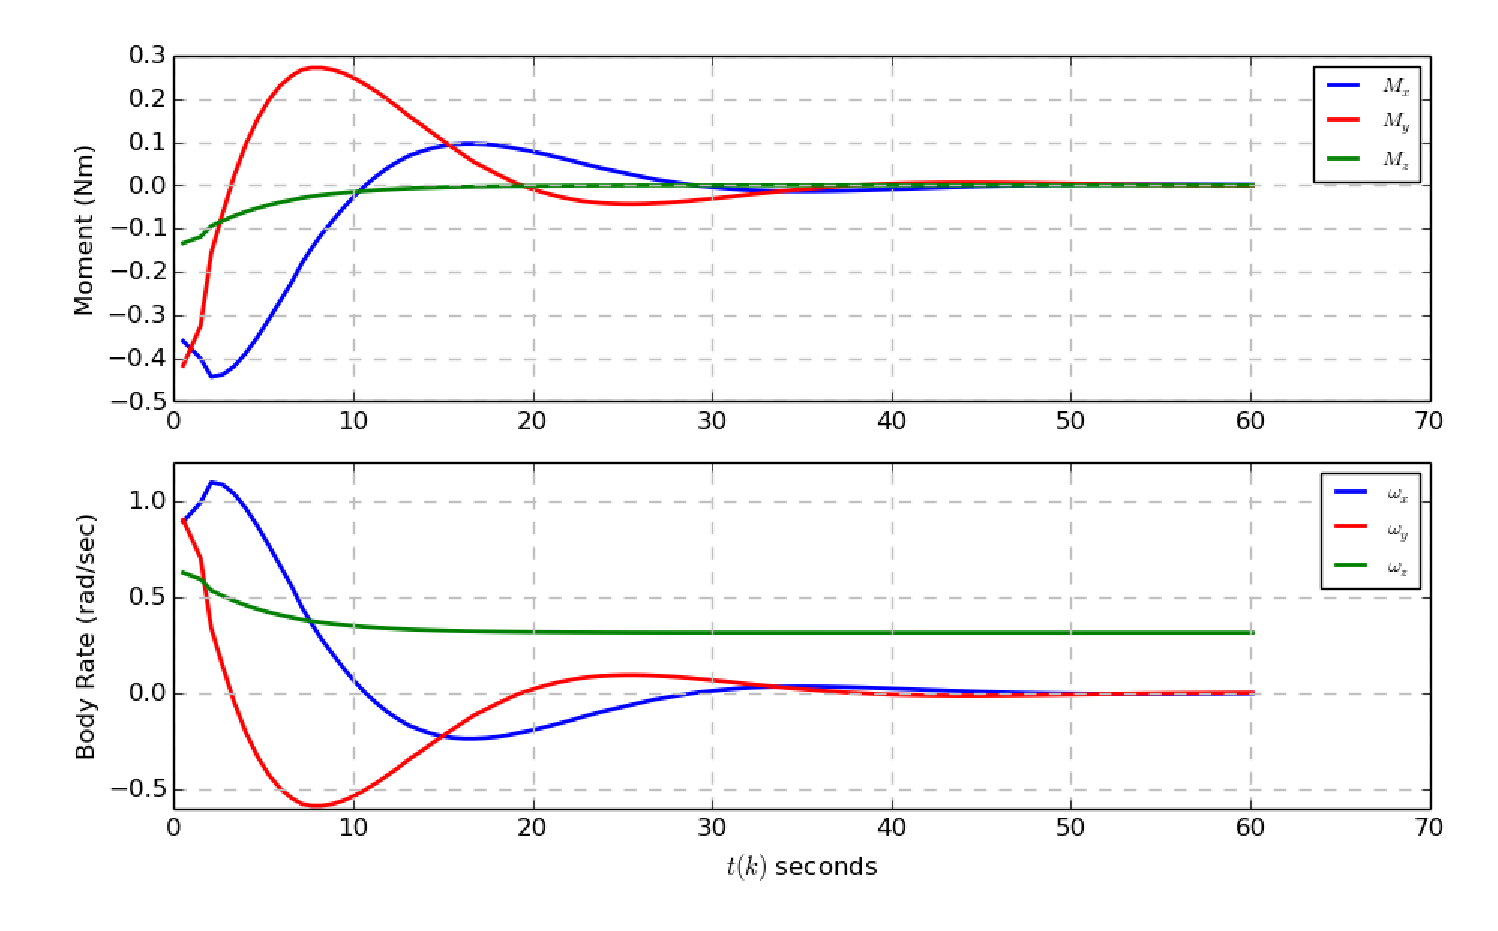
\psfig{file=figures/p_rate_control.eps,width=6in}}
  \caption{P rate control}
  \label{fig:PRateControl}
\end{figure}

\subsection{PID Rate Controller}
\label{subsec:PIDRateControl}

Expanding the proportional controller to include the integral and derivative term as shown in Equation (\ref{eqn:PIDRateControl}) can improve the performance slightly in tests with perfect measurement tests, but more importantly provides tools for dealing with noisy measurements when assessing observer-based controllers in Chapter \ref{chap:ObserverBasedControls}.  The integral and derivative terms are implemented with the $\Delta t_k$ adaptive step, as with the PID estimator, to help take into account inconsistencies in update intervals by tracking the step size at each update the resulting control algorithm is
\begin{equation}
  \begin{aligned}
    \bs{M}_{\omega} &= \bs{K}_{\omega p} \bs{\omega}_e + \bs{K}_{\omega i} \cdot (\Delta t_k \bs{I})\cdot \bs{\omega}_e + \bs{K}_{\omega d} \cdot \left(\frac{1}{\Delta t_k} \bs{I}\right) \cdot \bs(\bs{\omega}_e(t_k) - \bs{\omega}_e(t_{k-1}))
  \end{aligned}
  \label{eqn:PIDRateControl}
\end{equation}
\begin{figure}[H]
  \centerline{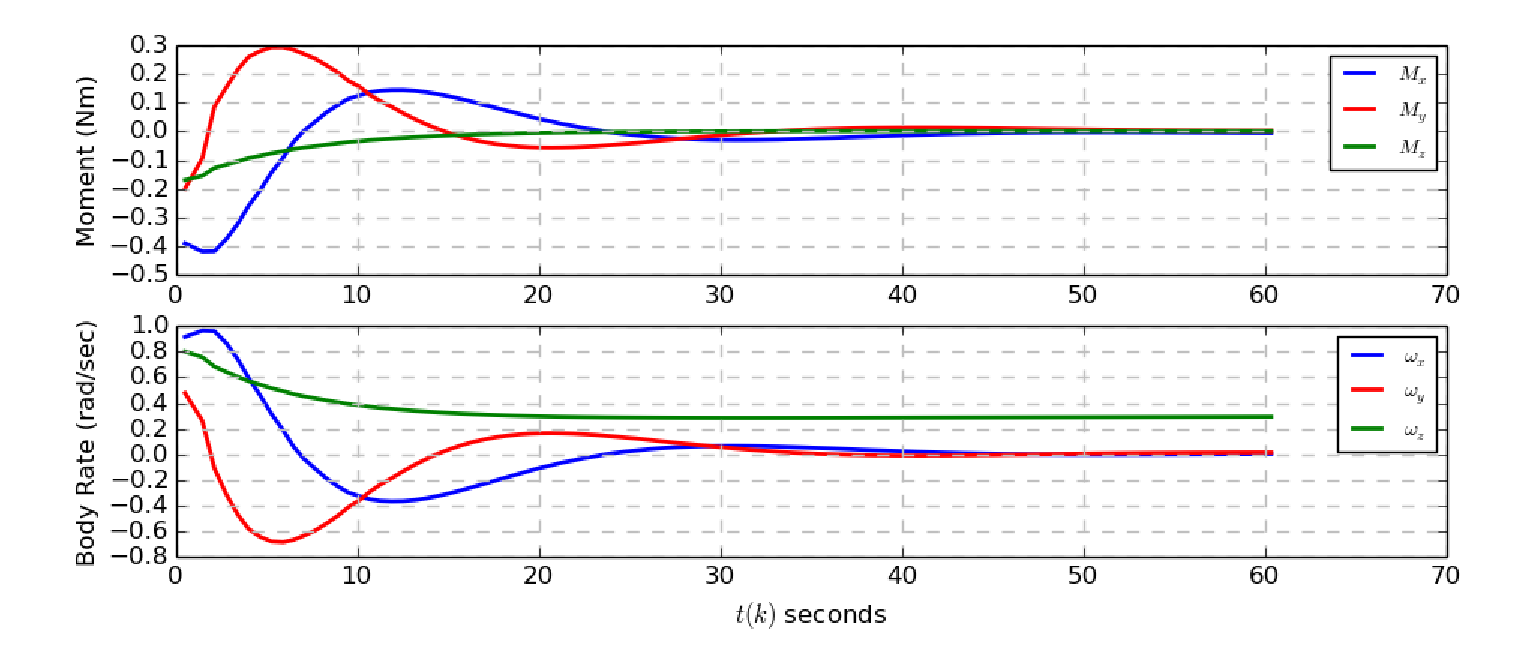
\psfig{file=figures/pid_rate_control.eps,width=6in}}
  \caption{PID rate control}
  \label{fig:PIDRateControl}
\end{figure}
The response curve in Figure \ref{fig:PIDRateControl} is generated from a random set of initial condition, and with the PID gains of Equation (\ref{eqn:PIDRateControlGains}) tuned through gradient descent iterations based on minimizing the total control effort.  In the case of perfect measurements, the two addition correctional control terms generally reduce the overshoot of the response but do not significantly decrease the settling time.
\begin{equation}
  \begin{aligned}
    \bs{K}_{\omega p} &= \begin{bmatrix} 0.424 & 0 & 0 \\ 0 & 0.416 & 0 \\ 0 & 0 & 0.346 \end{bmatrix},
    \bs{K}_{\omega i} = \begin{bmatrix} 0.006 & 0 & 0 \\ 0 & 0.003 & 0 \\ 0 & 0 & 0.005 \end{bmatrix} \\
    \bs{K}_{\omega d} &= \begin{bmatrix} 0.044 & 0 & 0 \\ 0 & 0.072 & 0 \\ 0 & 0 & 0.042 \end{bmatrix}
  \end{aligned}
  \label{eqn:PIDRateControlGains}
\end{equation}
Figure \ref{fig:PIDRateControlMoments} shows how the moments from each of the PID components contribute to the overall moments applied.  The addition of the derivative term gives the system a slightly quicker response than that with just the P-controller.   In this perfect measurement scenario the overall performance of the system would benefit from the integral term being removed altogether since it does not contribute much to the initial response and even causes a larger steady state error than the P-controller.
\begin{figure}[H]
  \centerline{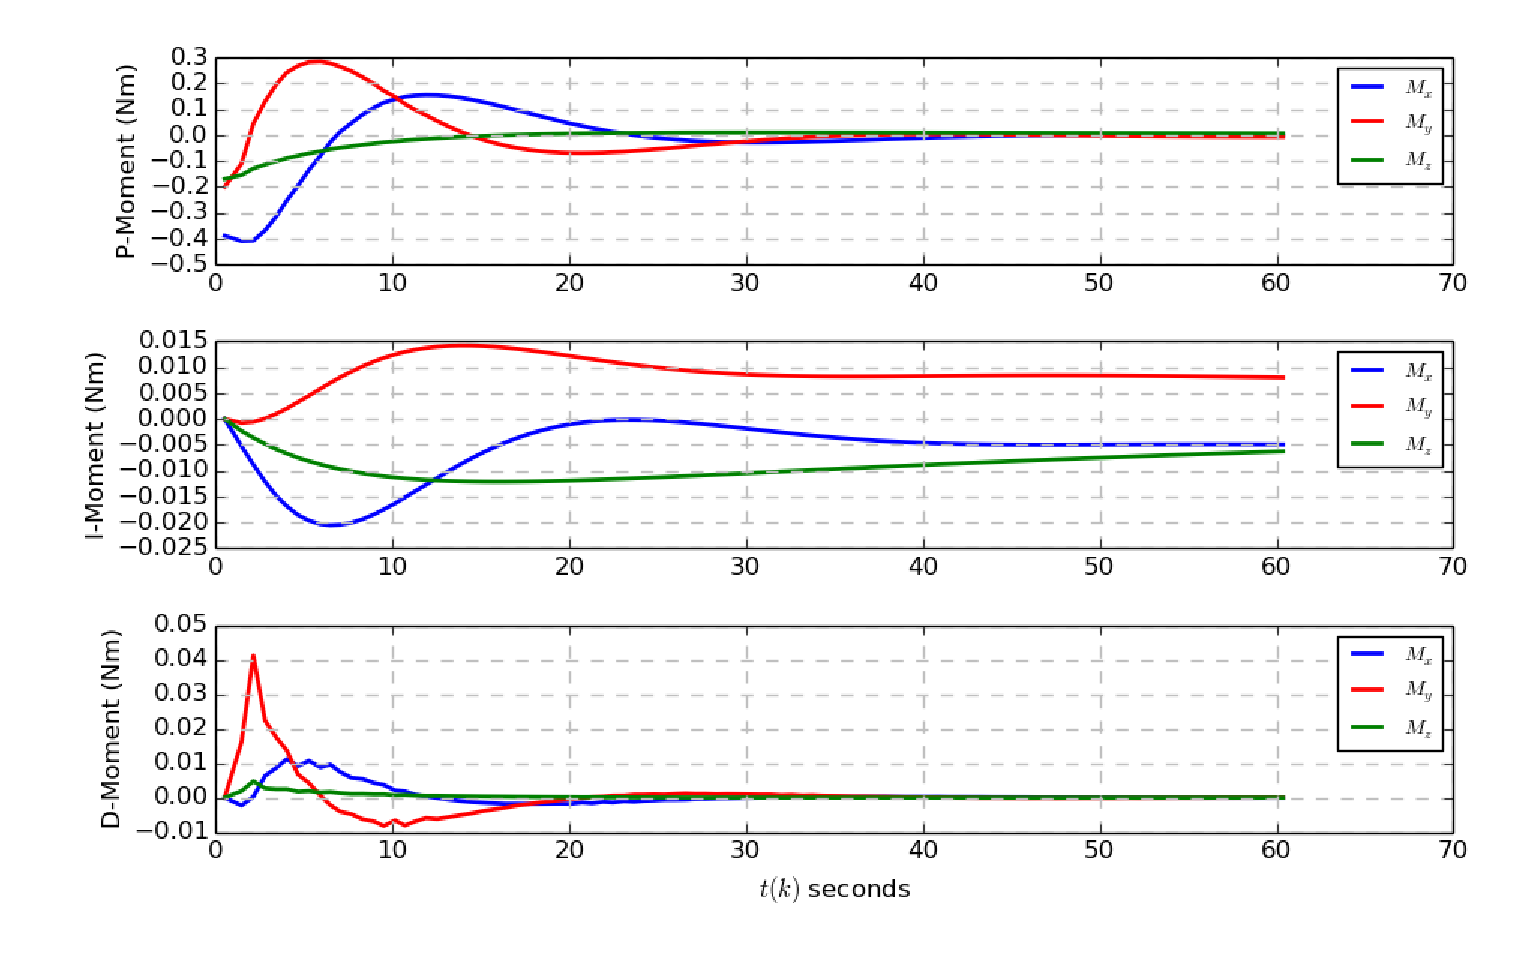
\psfig{file=figures/pid_rate_control_moments.eps,width=6in}}
  \caption{PID rate control moments}
  \label{fig:PIDRateControlMoments}
\end{figure}

\subsection{Sliding Mode Controller}
\label{subsec:SlidingModeController}

The Sliding Mode Controller (SMC) operates similarly to a proportional controller and is governed by the equation
\begin{equation}
  \bs{M}_{\omega} = \bs{L}_{\omega} \bs{\omega}_e + \bs{K}_{\omega}\bs{1}_s \big(\bs{\omega}_e \big)
  \label{eqn:SMController}
\end{equation}
where $\bs{L}_{\omega}$ is the proportional switching gain and the $\bs{1}_s$ function is a switching finction that can take a number of forms, such as the signum and arctangent functions.  In this thesis, the SMC uses the saturation function such that $\bs{1}_s$ is
\begin{equation}
  \bs{1}_s \big(\bs{\omega}_e \big) = sat \begin{bmatrix} \omega_{ex} / S_{\omega} &0 &0 \\ 0 & \omega_{ey} / S_{\omega} & 0 \\ 0 & 0 & \omega_{ez} / S_{\omega} \end{bmatrix}
\end{equation}
The SMC response in Figures \ref{fig:SMCRateControl} and \ref{fig:SMCRateControlMoments}, is generated with the following gain values tuned through a gradient descent search that minimizes control effort.
\begin{equation}
    \bs{L}_{\omega} = \begin{bmatrix} 0.3983 & 0 & 0 \\ 0 & 0.3828 & 0 \\ 0 & 0 & 0.4160 \end{bmatrix},
    \bs{K}_{\omega} = \begin{bmatrix} 0.4399 & 0 & 0 \\ 0 & 0.5097 & 0 \\ 0 & 0 & 0.3162 \end{bmatrix},
    S_{\omega} = 0.1404
  \label{SMCRateControlGains}
\end{equation}
The response to the test configuration shows significant improvements in performance over the P and PID rate controller as shown if Figure \ref{fig:SMCRateControl}, but at the cost of higher moment couple.
\begin{figure}[H]
  \centerline{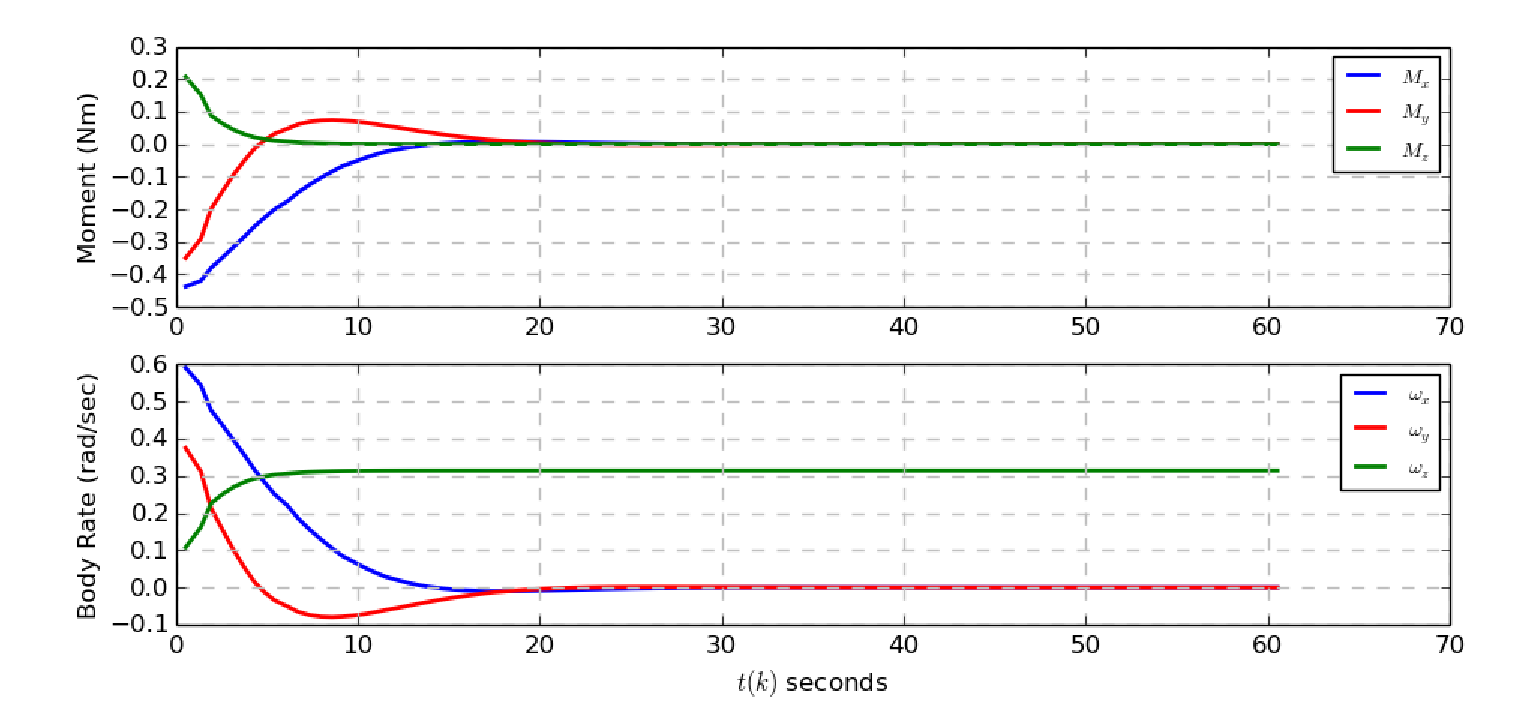
\psfig{file=figures/smc_rate_control.eps,width=6in}}
  \caption{SMC rate control}
  \label{fig:SMCRateControl}
\end{figure}
The moment graph in Figure \ref{fig:SMCRateControl} is a combination of the two terms in the SMC.  Breaking those overall moment values into the separate term's contributions (Figure \ref{fig:SMCRateControlMoments}) shows the similar profile between the proportional and saturation term contributions with the exception of the peaks missing from the saturation response.
\begin{figure}[H]
  \centerline{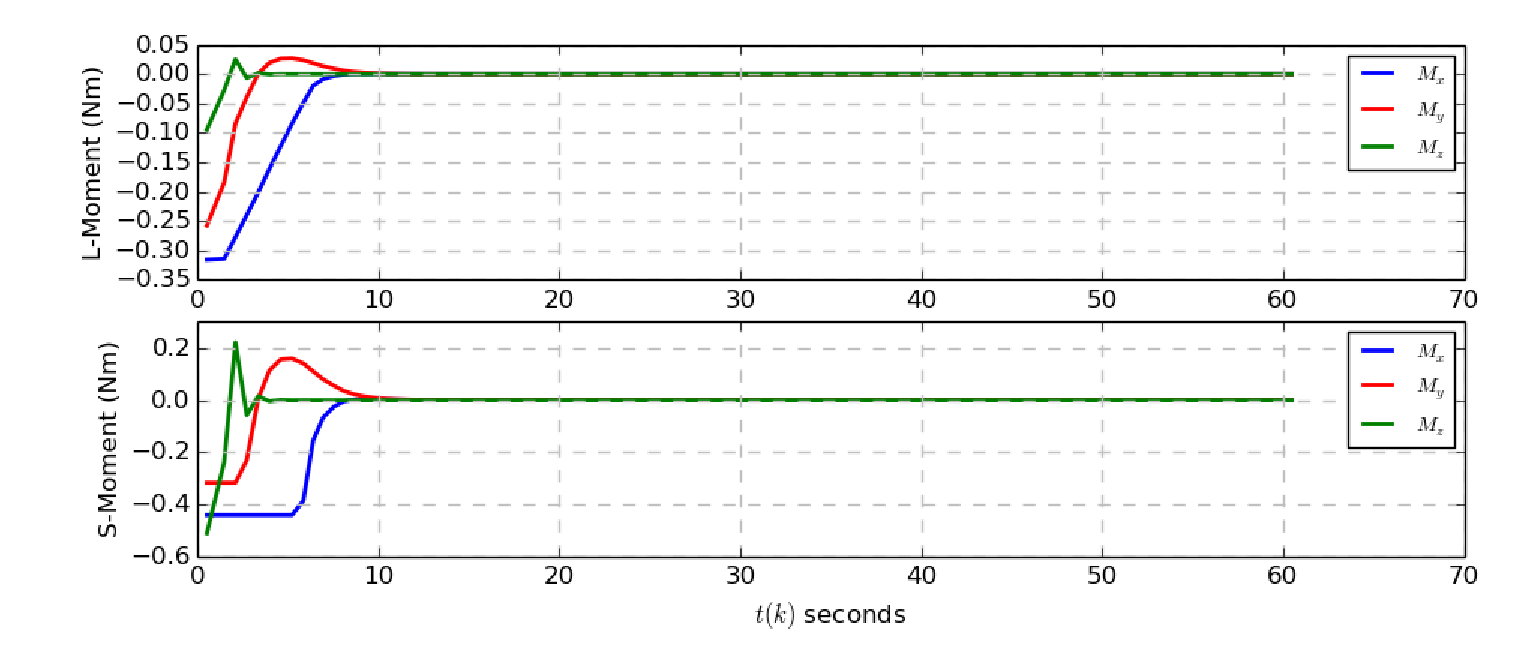
\psfig{file=figures/smc_rate_control_moments.eps,width=6in}}
  \caption{SMC rate control moments}
  \label{fig:SMCRateControlMoments}
\end{figure}
With assumed perfect state feedback, the saturation term adds a significant performance improvement over the P and PID implementations.  Additionally, with two fewer design gains, tuning the SMC is slightly less involved than the PID body rate controller.

\section{Quaternion to Moment Conversion}
\label{sec:QuaternionToMomentConversion}

The remainder of this chapter focuses on the attitude control problem to correct for nutation (Section \ref{sec:AttitudeAndNutationControl}) and the integration of the attitude and rate controller (Section \ref{sec:AttitudeandBodyRateControl}).  The proper conversion from an attitude error measurement to actuator moments is critical to providing a robust control method.

The attitude error measurement is calculated through the quaternion multiplicative method as is established in Section \ref{sec:HighIntegrityStateAdjustments}:

\begin{equation}
  \bs{q}_e = \bs{q}_d^* \otimes \bs{\hat{q}}
\end{equation}

Unlike with the estimator where the input and output formats are both quaternions, the quaternion error in the controller $\bs{q}_e$ is composed of four parameters that need to map to three moments values.  The commonly used method for this is to fall back on matrix algebra where $\bs{K}_q \in \Re^{3x4}$

\begin{equation}
  \bs{M}_q = \begin{bmatrix} 3 \times 4 \end{bmatrix} \begin{bmatrix} q_1 & q_2 & q_3 & q_0 \end{bmatrix}^T
  \label{eqn:traditional_attitude_controller}
\end{equation}

There are two main issues with this approach.  First, the quaternion parameters are sinusoidal in nature.  As such, during the conversion to moment values through matrix multiplication, the magnitude of the moment does not scale linearly with that of the attitude error.

The second issue is that the quaternion is comprised of a vector and scalar that provide two separate types of information about the attitude error.  Lumping the two together in a single matrix multiplication operation ignores the physical representation of their values.  The vector defines the Euler axis which gives the attitude error its direction.  A vector component with $q_1 = q_3 = 0, q_2 \ne 0$ means that to move the estimated satellite attitude to the desired attitude requires a rotation about just the body-fixed $y$-axis which requires a moment couple in just $M_y$.  This can be represented simply as
\begin{equation}
  \bs{M}_{q} = k\bs{v}_e
\end{equation}
This provides a basis for the direction of the moment couple.  However, since the rotational quaternion is fixed at a unit norm, the magnitude of the vector component $\bs{v}_e$ varies with the size of the error.  This is compensated for by normalizing the vector such that the moment is now chosen to equal
\begin{equation}
  \bs{M}_{q} = k\bs{\hat{e}}_e
  \label{eqn:quat_vector_to_moment}
\end{equation}
where $\bs{\hat{e}}_{e}$, the Euler axis, is the normalized vector component of the quaternion.

With Equation (\ref{eqn:quat_vector_to_moment}) establishing the direction of the axis of the actuator moments, one now needs only to determine how to scale the moment couples in relation to the size of the error.  The remaining $q_0$ quantity is a reasonable first choice and the moment is now chosen to equal
\begin{equation}
  \bs{M}_{q} = kq_{0e} \bs{\hat{e}}_e
\end{equation}
where $q_{0en}$ is the scalar component of the error quaternion.

$q_{0e}$, as with the vector, is a sinusoidal measure.  The underlying rotation angle $\theta$ measure of the quaternion rotation, however, is a direct measure of the attitude error.  Extracting $\theta$ measure from $q_{0e}$ and incorporating into the moment calculation yields a final choice of $\bs{M}_q$ such that
\begin{equation}
  \begin{aligned}
    \bs{M}_{q} &= k \theta \bs{\hat{e}}_e \\
    \bs{M}_{q} &= \left[- 2k \cos^{-1} (q_{0e}) \right] \bs{\hat{e}}_e
  \end{aligned}
  \label{eqn:QuaternionToMomentConversion}
\end{equation}
where $q_{0e} = \cos(-\theta_e/2)$ from the definition of a rotational quaternion.

This conversion is used throughout all attitude control calculations in the remainder of this thesis.








\section{Attitude and Nutation Control}
\label{sec:AttitudeAndNutationControl}

Section \ref{sec:RateControl} covered the design of the rate controller which addresses the first controller goal to maintain a spin rate of $\omega_z = 3$ rpm.  This section ignores the rate control requirement and focuses strictly on the attitude control problem by incorporating the quaternion to moment conversion of Equation (\ref{eqn:QuaternionToMomentConversion}) into a PID and SMC attitude controller.   Later, Section \ref{sec:AttitudeandBodyRateControl} combines the attitude and body rate controls into a single controller.

\subsection{P Attitude Control}
\label{subsec:PAttitudeControl}

Starting with a simplest design of the proportional attitude control, Equation (\ref{eqn:QuaternionToMomentConversion}) can be directly applied as
\begin{equation}
  \bs{M}_{q} = \left[- 2K_{qp} \cos^{-1} \big(q_{0e} \big) \right] \bs{\hat{e}}_e \\
  \label{eqn:PAttitudeControl}
\end{equation}
This format of the proportional controller provides a significant time savings over the traditional method described in Equation (\ref{eqn:traditional_attitude_controller}), the number of design gains is reduced from 12 gain values to tune to a single gain.

To assess the accuracy of implementation, an example is analyzed through the use of TSatPy.  A system is initialized to a state of
\begin{equation}
  \bs{x}_0 = \begin{bmatrix} 0 \bs{i} -0.0477 \bs{j} -0.477 \bs{k} +0.8778 \\ 0 \bs{i} -0.01 \bs{j} +0.2 \bs{k} \end{bmatrix}
\end{equation}
which is essentially a 1 radian rotation about the $z$-axis with a small nutation such that initial $\omega_y = -0.01$ rad/sec.  The controller,s desired state is to return to the standard attitude where the body-fixed reference frame is aligned with that of the global reference frame
\begin{equation}
  \bs{q}_d = 0 \bs{i} +0 \bs{j} +0 \bs{k} + 1
\end{equation}
The chosen proportional gain is given as
\begin{equation}
  K_{qp} = 0.04
\end{equation}
The results from the test are shown in Figure \ref{fig:PAttitudeControl}.  The total simulation time is 120 seconds.  The top graph displays the calculated moments required to compensate for the attitude error.  As expected, $M_z$ responds in the sinusoidal pattern as the P-controller overshoots the desired attitude.  The center graph displays $\theta$ and quantifies the distance between the current and desired attitude.  With this measure, it is seen that while the majority of the attitude error is linked to the rotation about the $z$-axis.  The error progressively increases through each rotation as some of the rotational motion is transferred to the out-of-plane motion (i.e. nutation).
\begin{figure}[H]
  \centerline{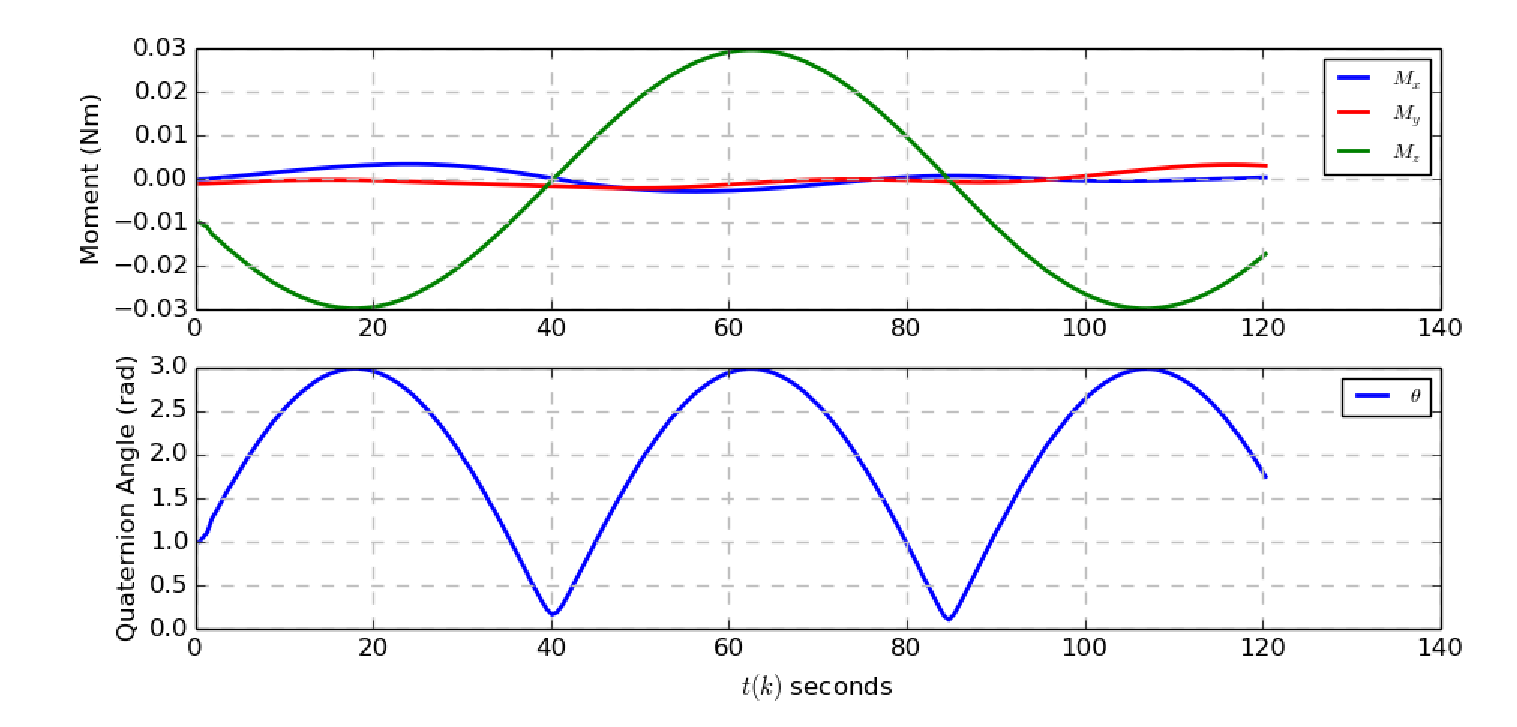
\psfig{file=figures/p_attitude_control.eps,width=6in}}
  \caption{P Attitude Control}
  \label{fig:PAttitudeControl}
\end{figure}



\subsection{Quaternion Decomposition for Nutation Control}
\label{subsec:QuaternionDecompositionForNutationControl}

Prior to combining attitude control from Section \ref{subsec:PAttitudeControl} with body rate control from Section \ref{sec:RateControl}, the controller needs to incorporate the quaternion decomposition method of Equation (\ref{eqn:quaternion_decomposition_derivation}).  The advantage to incorporating this into a controller is being able to take the quaternion portion of the state error, decompose it into its associated rotation and nutation quaternions, and replace quaternion error with the corresponding nutational quaternion error.  This attitude controller, thus, need only correct for nutation, regardless of the attitude or angular velocity.

The proportional attitude control from Equation (\ref{eqn:PAttitudeControl}) becomes
\begin{equation}
  \bs{M}_{q} = \left[-2 K_{qp} \cos^{-1} \big(q_{0en} \big) \right] \bs{\hat{e}}_{en} \\
\end{equation}
where $q_{0en}$ is the scalar component of the error quaternion's nutation component, and $\bs{\hat{e}}_{en}$ is the normalized Euler axis for the nutation component.

Snippet \ref{code:nut_from_quat} shows how with TSatPy the nutation component of the quaternion can be extracted from the state quaternion for use in moment calculations.

\begin{listing}[H]
\begin{singlespace}
  \begin{minted}[mathescape,linenos,numbersep=10pt,frame=lines,framesep=2mm]{python}
from TSatPy.State import State, Quaternion, BodyRate

print("State Error")
x_e = State(
    Quaternion([0,0.1,1],radians=1),
    BodyRate([0,-0.01,0.2]))
print("x_e: %s" % (x_e))

print("Decomposed Quaternion")
q_r, q_n = x_e.q.decompose()
print("q_r: %s" % q_r)
print("q_n: %s" % q_n)

print("Nutation Only State Error")
x_e.q = q_n
print("x_e: %s" % (x_e))

# Prints Out
# State Error
# x_e: <Quaternion [-0 -0.0477046 -0.477046], 0.877583>,
#      <BodyRate [0 -0.01 0.2]>
# Decomposed Quaternion
# q_r: <Quaternion [0 0 -0.47759], 0.878583>
# q_n: <Quaternion [-0.0227833 -0.0419125 -0], -0.998861>
# Nutation Only State Error
# x_e: <Quaternion [-0.0227833 -0.0419125 -0], -0.998861>,
#      <BodyRate [0 -0.01 0.2]>
  \end{minted}
\caption{Extracting the nutation quaternion from the state quaternion}
\label{code:nut_from_quat}
\nocite{minted}
\end{singlespace}
\end{listing}

\subsection{P Nutation Control}
\label{subsec:PNutationControl}

Using the proportional control
\begin{equation}
  \bs{M}_{q} = \left[- 2K_{qp} \cos^{-1} (q_{0n}) \right] \bs{\hat{e}}_n
  \label{eqn:PNutationControl}
\end{equation}
with the same initial state and desired quaternion as the proportional attitude controller from the previous example.  That is,
\begin{equation}
  \bs{x}_0 = \begin{bmatrix} 0 \bs{i} -0.0477 \bs{j} -0.477 \bs{k} +0.8778 \\ 0 \bs{i} -0.01 \bs{j} +0.2 \bs{k} \end{bmatrix}
\end{equation}
\begin{equation}
  \bs{q}_d = 0 \bs{i} +0 \bs{j} +0 \bs{k} + 1
\end{equation}
\begin{figure}[H]
  \centerline{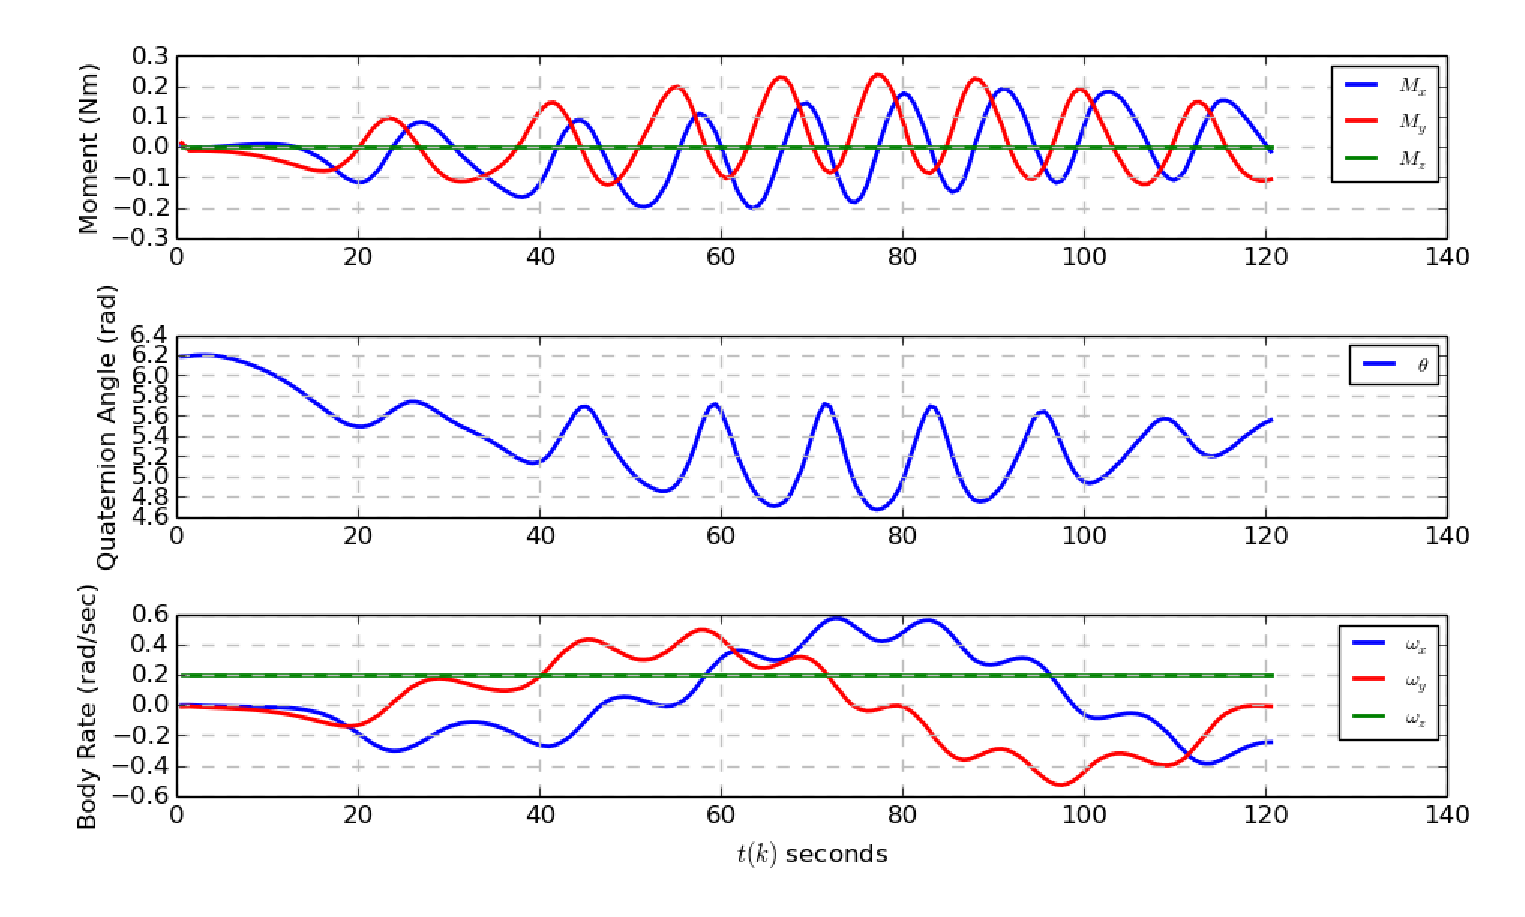
\psfig{file=figures/p_nutation_control.eps,width=6in}}
  \caption{P Nutation Control}
  \label{fig:PNutationControl}
\end{figure}
Figure \ref{fig:PNutationControl} shows the resulting control moments, quaternion angle error, and body rates with these conditions.  In the first and last plots, the body rates and moments show expected behavior, where the corrections for initial nutation cause fluctuations in $\omega_x$ and $\omega_z$ with $\omega_z$ remaining unchanged.  This means that for spin-stabilized systems like NASA's MMS Mission satellite, the controller can correct for nutation errors and is unaffected by the constant spin rate.  The same can be seen in the first graph where moments are applied about the $x$ and $y$ axes, but none are applied to control the initial spin about the $z$-axis.
The center plot tracking quaternion angle shows that while some of the nutation is removed, the proportional nutation controller is clearly not sufficient to remove all nutation.


\section{Attitude and Body Rate Control}
\label{sec:AttitudeandBodyRateControl}

Sections \ref{sec:RateControl} and \ref{sec:AttitudeAndNutationControl} have established methods to address spin rate and nutation control goals.  In this section the two are used together.  In Section \ref{subsec:FixedAttitudeControl}, the attitude and body rate controllers are combined to take a satellite from an initialized uncontrolled spin and detumble it to the standard orientation so that the body-fixed axes are aligned with the global axes.  Section \ref{subsec:SpinStabilizedControl} releases the restriction on motion about the $z$-axis and takes the satellite's initial uncontrolled spin to a nutation-free rotation about the $z$-axis.
\begin{equation}
    \bs{M} = \bs{M}_{q} + \bs{M}_{\omega}
\end{equation}
For consistency, all tests in this section are initialized with the following state
\begin{equation}
  \bs{x}_0 = \begin{bmatrix} -0.532 \bs{i} -0.417 \bs{j} -0.275 \bs{k} +0.684 \\ 0.315 \bs{i} +0.207 \bs{j} +0.113 \bs{k} \end{bmatrix}
  \label{eqn:attitude_and_body_rate_control_ic}
\end{equation}

\subsection{Fixed Attitude Control}
\label{subsec:FixedAttitudeControl}
The PID controllers are defined as
\begin{equation}
  \begin{aligned}
    \bs{M} &= \bs{M}_{q} + \bs{M}_{\omega} \\
    \bs{M}_{q} &= \left[- 2K_{qp} \cos^{-1} (q_{0e}) \right] \bs{\hat{e}}_e + \left[- 2K_{qi} \cos^{-1} (q_{0ei}) \right] \bs{\hat{e}}_{ei} + \left[- 2K_{qd} \cos^{-1} (q_{0ed}) \right] \bs{\hat{e}}_{ed} \\
    \bs{M}_{\omega} &= \bs{K}_{\omega p} \bs{\omega}_e + \bs{K}_{\omega i} \cdot (\Delta t_k \bs{I})\cdot \bs{\omega}_e + \bs{K}_{\omega d} \cdot \left(\frac{1}{\Delta t_k} \bs{I}\right) \cdot (\bs{\omega}_e(t_k) - \bs{\omega}_e(t_{k-1}))
  \end{aligned}
\end{equation}
where $\bs{\hat{e}}_e, \bs{\hat{e}}_{ei}, \text{ and } \bs{\hat{e}}_{ed}$ are the Euler axes for the quaternion error, quaternion error integral, and quaternion error derivative, respectively, with the integral $\bs{q}_{ei}$ and derivative $\bs{q}_{ed}$ quaternions from Equations (\ref{eqn:IEstimator}) and (\ref{eqn:DEstimator}).

The results from the PID body rate and attitude controller are shown in Figures \ref{fig:PIDAttitudeAndRateControl} and \ref{fig:PIDAttitudeAndRateControlMoments} and are tested with the following control gains:
\begin{equation}
  \begin{aligned}
    K_{qp} &= 0.6022,K_{qi} = 0.04656,K_{qd} = 0.8554 \\
    K_{\omega p} &= \bs{I} \begin{bmatrix} 0.70326 & 0.7203 & 0.61757 \end{bmatrix}^T \\
    K_{\omega i} &= \bs{I} \begin{bmatrix} 0.04207 & 0.06999 & 0.018591 \end{bmatrix}^T \\
    K_{\omega d} &= \bs{I} \begin{bmatrix} 0.4096 & 0.6032 & 0.6123 \end{bmatrix}^T
  \end{aligned}
\end{equation}
\begin{figure}[H]
  \centerline{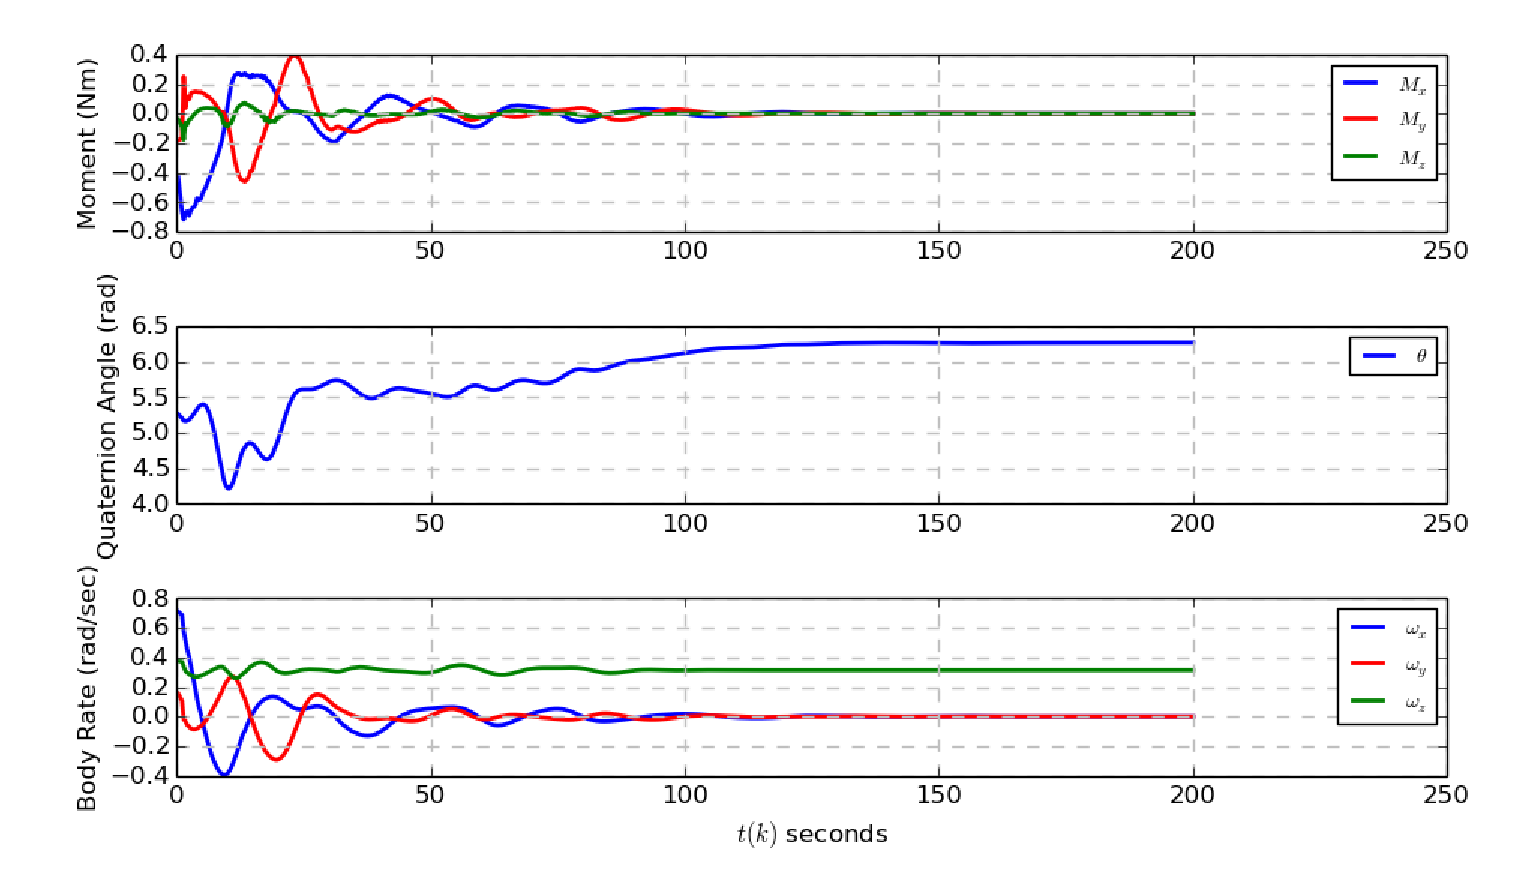
\psfig{file=figures/pid_attitude_and_rate_control.eps,width=6in}}
  \caption{PID Attitude and Rate Control}
  \label{fig:PIDAttitudeAndRateControl}
\end{figure}
Figure \ref{fig:PIDAttitudeAndRateControl} shows a significant improvement in the body rate control response over previous body rate tests.  All error and oscillations in the quaternion angle are also eliminated.  The proportional, integral, and derivative terms that comprise the moment value from Figure \ref{fig:PIDAttitudeAndRateControl} are shown individually in Figure \ref{fig:PIDAttitudeAndRateControlMoments}.
\begin{figure}[H]
  \centerline{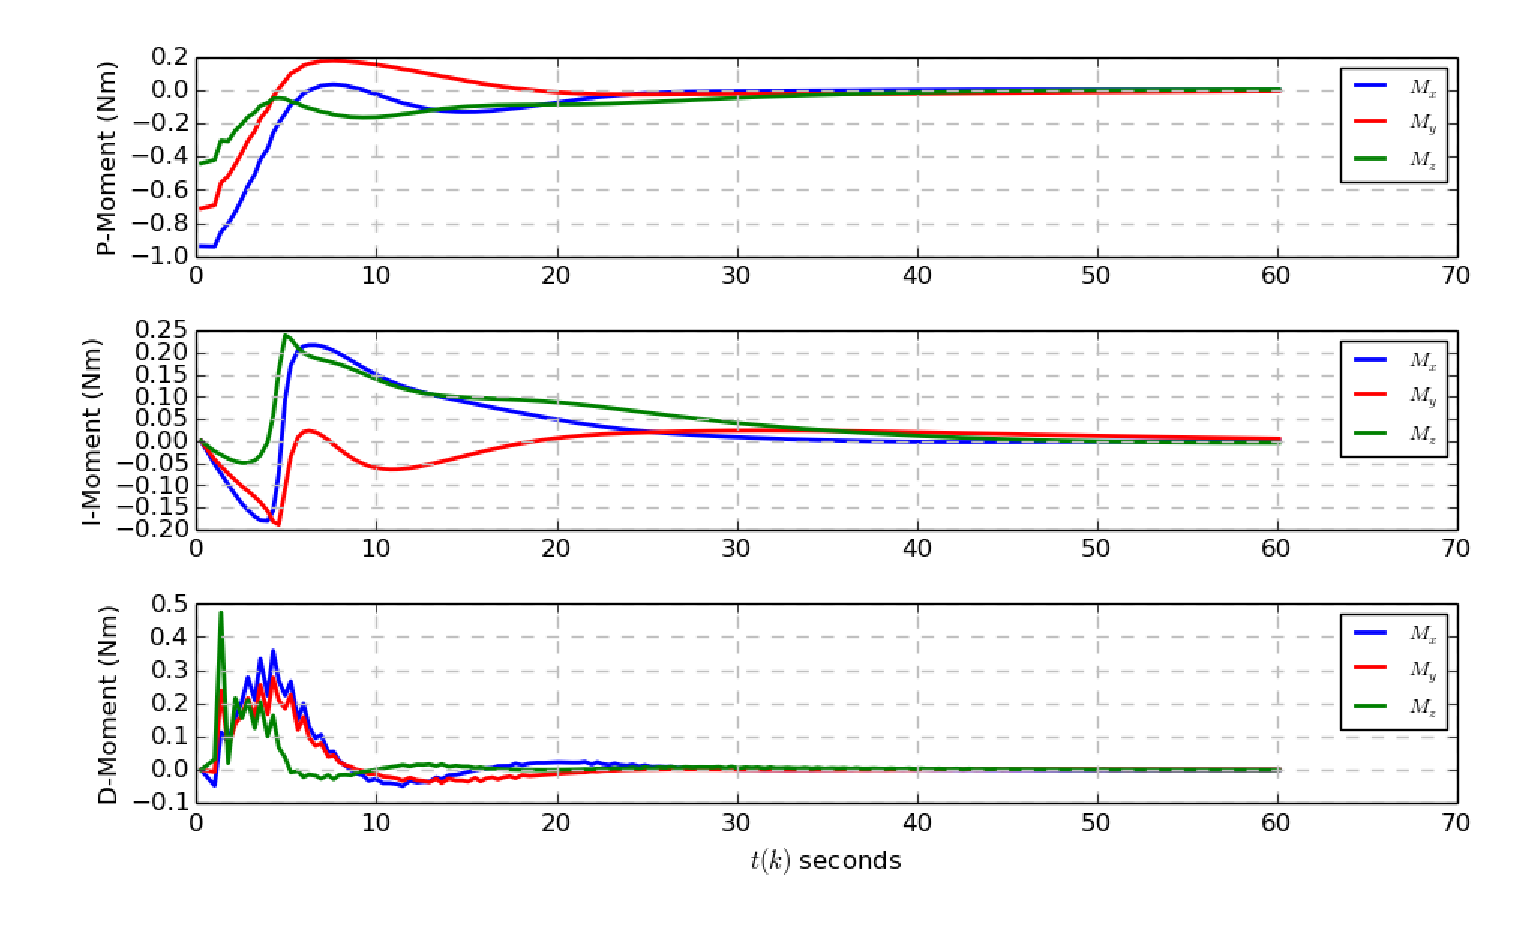
\psfig{file=figures/pid_attitude_and_rate_control_moments.eps,width=6in}}
  \caption{PID Attitude and Rate Control Moments}
  \label{fig:PIDAttitudeAndRateControlMoments}
\end{figure}

The Sliding Mode Controller is designed such that
\begin{equation}
  \begin{aligned}
    \bs{M} &= \bs{M}_{q} + \bs{M}_{\omega} \\
    \bs{M}_{q} &= \left[- L_{q} \cos^{-1} (q_{0e}) \right] \bs{\hat{e}}_e + \left[ K_{q} sat \left( \frac{-2\cos^{-1} (q_{0e})}{S_q} \right) \right] \bs{\hat{e}}_e \\
    \bs{M}_{\omega} &= \bs{L}_{\omega} \bs{\omega}_e + \bs{K}_{\omega}\bs{1}_s \big(\bs{\omega}_e / S_{\omega} \big) \\
    \bs{1}_s \big(\bs{\omega}_e / S_{\omega} \big) &= \begin{bmatrix} sat (\omega_{ex} / S_{\omega}) &0 &0 \\ 0 & sat (\omega_{ey} / S_{\omega}) & 0 \\ 0 & 0 & sat (\omega_{ez} / S_{\omega}) \end{bmatrix}
  \end{aligned}
  \label{eqn:sliding_mode_control}
\end{equation}
Where $S_{\omega}$ represents the boundary layer for the saturation functions.

Figures \ref{fig:SMCAttitudeAndRateControl} and \ref{fig:SMCAttitudeAndRateControlMoments} show the response of the SMC for attitude and body rate control.  Through a gradient descent search, the SMC parameters are tuned to
\begin{equation}
  \begin{aligned}
    L_q &= 0.408, \bs{L}_{\omega} = \bs{I} \begin{bmatrix} 0.708 & 0.678 & 0.525 \end{bmatrix}^T \\
    K_q &= 0.500, \bs{K}_{\omega} = \bs{I} \begin{bmatrix} 0.745 & 0.816 & 0.666 \end{bmatrix}^T \\
    S_q &= 0.607, S_{\omega} = 0.315
  \end{aligned}
\end{equation}
\begin{figure}[H]
  \centerline{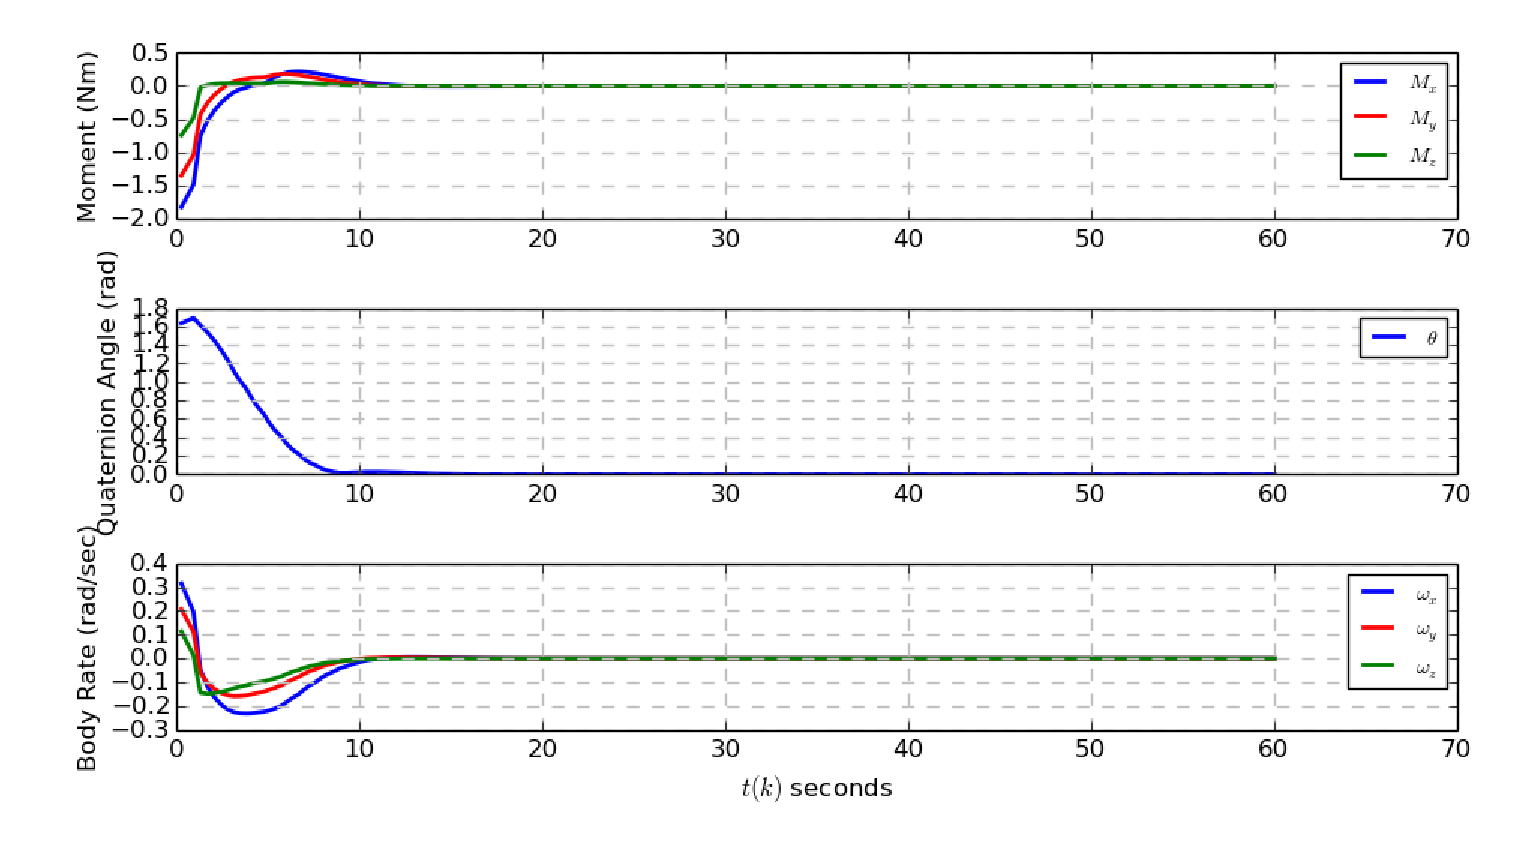
\psfig{file=figures/smc_attitude_and_rate_control.eps,width=6in}}
  \caption{SMC Attitude and Rate Control}
  \label{fig:SMCAttitudeAndRateControl}
\end{figure}
\begin{figure}[H]
  \centerline{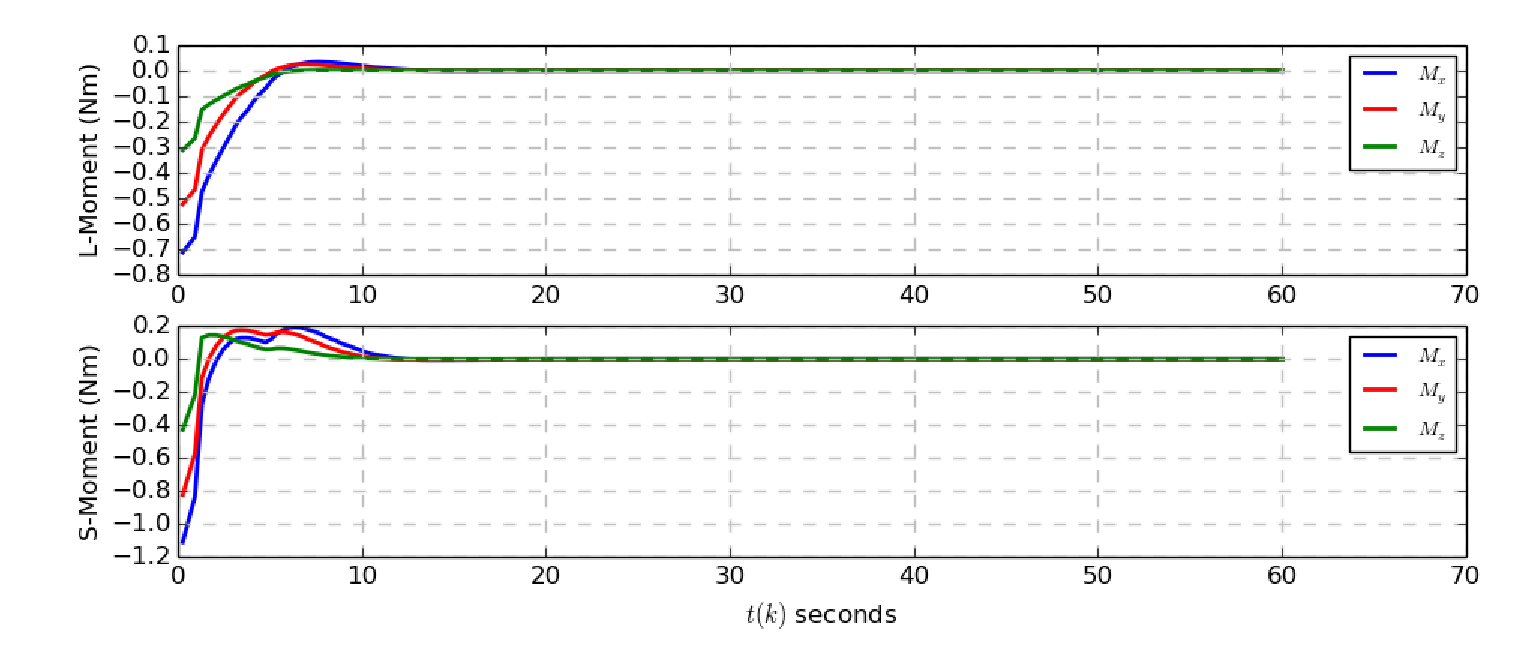
\psfig{file=figures/smc_attitude_and_rate_control_moments.eps,width=6in}}
  \caption{SMC Attitude and Rate Control Moments}
  \label{fig:SMCAttitudeAndRateControlMoments}
\end{figure}
As with the body rate comparative tests, the SMC shows a significant improvement in performance compared to the PID controller for fixed attitude and body control.

\subsection{Spin-Stabilized Control}
\label{subsec:SpinStabilizedControl}

For the fixed attitude control problem from Section (\ref{subsec:FixedAttitudeControl}), this section verifies the ability of a controller to release the quaternion restriction on the rotational attitude leaving the system to control five degrees of freedom: $\omega_z = 0.314, \omega_x = \omega_y = 0$ and zero nutation about the $x$ and $y$ axes.  Since the Sliding Mode Controller regularly out performs the PID controller, the spin-stabilized controller will run with control Equation (\ref{eqn:sliding_mode_control}) using the following controller gains:
\begin{equation}
  \begin{aligned}
    L_q &= 0.01, \bs{L}_{\omega} = \bs{I} \begin{bmatrix} 0.398 & 0.383 & 0.416 \end{bmatrix}^T \\
    K_q &= 0.01, \bs{K}_{\omega} = \bs{I} \begin{bmatrix} 0.440 & 0.510 & 0.316 \end{bmatrix}^T \\
    S_q &= 0.01, S_{\omega} = 0.140
  \end{aligned}
\end{equation}

The initial convergence of the spin-stabilized state takes place quickly, as in previous test configurations.  In this case, however, the controller is not able to fully remove the attitude error.  Additional gain tuning or the inclusion of advanced visualizations such as the tPlot discussed in Section \ref{sec:ObjectOrientedNSSControlSystem} is required to diagnose the source of the error.
\begin{figure}[H]
  \centerline{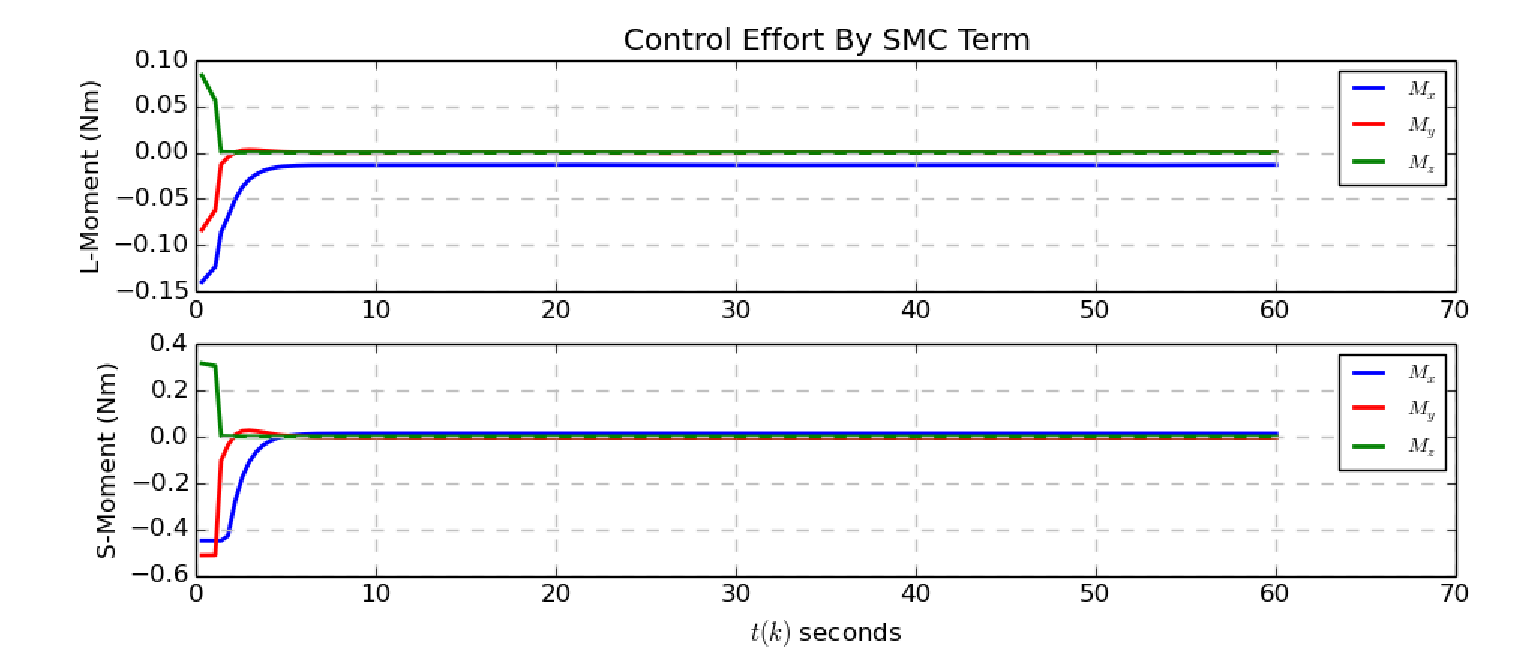
\psfig{file=figures/smc_nutation_and_rate_control.eps,width=6in}}
  \caption{SMC Nutation and Rate Control}
  \label{fig:SMCNutationAndRateControl}
\end{figure}
\begin{figure}[H]
  \centerline{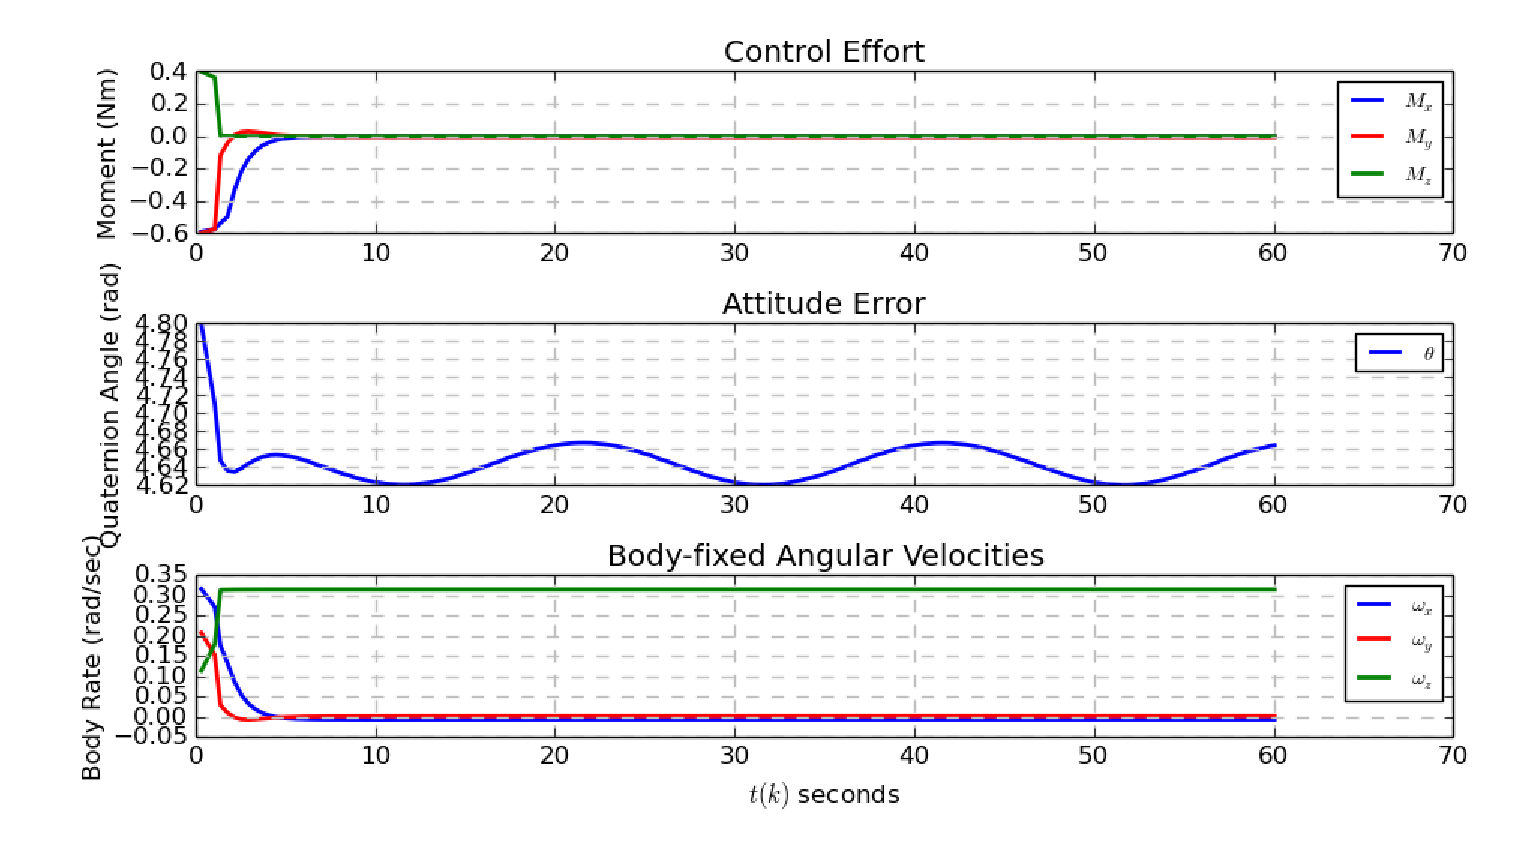
\psfig{file=figures/smc_nutation_and_rate_control_moments.eps,width=6in}}
  \caption{SMC Nutation and Rate Control Moments}
  \label{fig:SMCNutationAndRateControlMoments}
\end{figure}
